\documentclass[a4paper]{article}

\usepackage{INTERSPEECH2016}
\usepackage{graphicx}
\usepackage{amssymb,amsmath,bm}
\usepackage{textcomp}
\usepackage{epsfig,amsmath,rotating,latexsym,comment}
\usepackage{subfigure,tabularx,tabulary,caption,float}
\usepackage{enumitem} % remove tab for bullet points during itemize
\usepackage[noadjust]{cite} % to produce ranges [1]-[3] instead of [1],[2],[3] and to sort the order
\usepackage{color}
\usepackage{tikz}
\usepackage{tipa}\newcommand{\ipa}[1]{\textipa{#1}}
\usepackage{stackrel}
%\usepackage{wrapfig} % remove whitespace around fig
%\usepackage{lipsum}
\usetikzlibrary{positioning,shadows,arrows,shapes,calc}
%\usepackage{graphicx,pstricks}
%\usepackage{cases}
\def\vec#1{\ensuremath{\bm{{#1}}}}
\def\mat#1{\vec{#1}}
\DeclareMathOperator*{\argmax}{arg\,max}
\DeclareMathOperator*{\argmin}{arg\,min}
\newcommand{\mytikzscale}{0.8}
\newcommand{\myvspacefig}{\vspace{-4mm}}

\sloppy % better line breaks
\ninept

\title{An investigation on training deep neural networks using probabilistic transcriptions}

\makeatletter
\def\name#1{\gdef\@name{#1\\}}
\makeatother \name{{\em Amit Das, Mark Hasegawa-Johnson}}

\address{Department of Electrical and Computer Engineering \\
University of Illinois at Urbana-Champaign \\
Illinois, IL 61801, USA \\
{\small \tt \{amitdas, jhasegaw\}@illinois.edu}}


\begin{document}
\maketitle

\begin{abstract}
In this study, a transfer learning technique is presented for cross-lingual speech recognition in an adverse  scenario where there are no natively transcribed transcriptions in the target language. The transcriptions that are available during training are transcribed by crowd workers who neither speak nor have any familiarity with the target language. Hence, such transcriptions are likely to be inaccurate. Training a deep neural network (DNN) in such a scenario is challenging; previously reported results have described DNN error rates exceeding the error rate of an adapted Gaussian Mixture Model (GMM). This paper investigates multi-task learning techniques using deep neural networks which are suitable for this scenario.  We report, for the first time, absolute improvement in phone error rates (PER) in the range 1.3-6.2\% over GMMs adapted to probabilistic transcriptions. Results are reported for Swahili, Hungarian, and Mandarin.
\end{abstract}
%
\noindent{\bf Index Terms}: cross-lingual speech recognition, transfer learning, deep neural networks, probabilistic transcription
\vspace{-3mm}
%
\section{Introduction}  \vspace{-2mm}
\label{sec:Introduction}
%Transfer learning has been successfully implemented for semi-supervised learning \cite{Juihuang-PhDThesis, Huang2009SemisupervisedlearningHLT} and supervised learning \cite{Huang-CrossDialectArabic} of GMMs. 
We explore training deep neural networks using probabilistic transcripts (PT) but no deterministic transcripts (DT) in the target language. DT means the transcript was collected from native speakers of a language. Since there is no ambiguity in such ground truth labels, the labels are deterministic in nature. The labels are then converted to IPA phone symbols. As an example the DT for the word ``cat" can be represented as shown in Fig.~\ref{fig:dt} with each arc representing a symbol and a probability value. Here, each symbol occurs with probability 1.0. On the other hand, PT means that the transcript was probabilistic or ambiguous in nature. Such transcripts frequently occur, for example, when collected from crowd workers who do not speak the language they are transcribing \cite{Jyothi-MismatchedCrowdsourcingTrans}. Usually a training audio clip (in some language $L$) is presented to a set of crowd workers who neither speak $L$ nor have any familiarity with it. Thus, due to their lack of knowledge about $L$, the labels provided by such workers are inconsistent, i.e., a given segment of speech can be transcribed by a variety of labels. This inconsistency can be modeled as a probability mass function (pmf) over the set of labels transcribed by crowd workers. Such a pmf can be graphically represented by a confusion network as shown in Fig.~\ref{fig:pt}. Unlike the DT in Fig.~\ref{fig:dt} which has a single sequence of symbols, the PT has 3$\times$4$\times$3$\times$4 = 144 possible sequences, one of which could be the right sequence. In this case, it is ``\ipa{k} \ipa{\ae} $\emptyset$ \ipa{t}".

%This is further aggravated by the fact the workers are unlikely to transcribe a phone if it is outside their %native language but is part of the language $L$.

Collecting and processing PTs for audio data in the target language $L$ from crowd workers who do not understand $L$ is called \emph{mismatched crowdsourcing} \cite{Jyothi-MismatchedCrowdsourcingTrans}. The language $L$ is the language we want to recognize using an automatic speech recognition (ASR) system trained using PTs. The objective of this study is to train a deep neural network using PTs in language $L$ while transfering knowledge from DTs in other languages excluding $L$.  An ASR system trained this way is particularly useful for low-resourced languages where it is difficult to find native transcribers in $L$ but easy to find non-native crowd workers through online sources like Amazon's Mechanical Turk or Upwork. The following five low resource conditions outine the nature of the data used in this study:  \vspace{-1mm}
\begin{itemize}[leftmargin=*]
\item PTs in Target Language: PTs in the target language $L$ are collected from crowd workers who do not speak $L$. \vspace{-2mm}
\item PTs are limited: The amount of PTs available from the crowd workers is limited to only 40 minutes of audio.  \vspace{-2mm}
\item Zero DT in Target Language: There are no DTs in $L$.  \vspace{-2mm}
\item DTs only in Source Languages: There are DTs from 5 other languages ($\ne L$).  \vspace{-2mm}
\item DTs are limited: The DTs are worth about 40 minutes of audio per language. Hence, the total amount of multilingual DTs available for training is $\approx$ 3.3 hours. (40 minutes/language $\times$ 5 languages = 200 minutes)  \vspace{-1mm}
\item Unsupervised data in Target Language: There are at least 5 hours of unlabeled data in $L$.  \vspace{-1mm}
\end{itemize}
% Many interesting research studies on DNNs have improved the performance of cross-lingual speech recognition.  Recently, DNNs have spurred interest in the speech recognition community due to their superior discriminative modeling capabilities  compared to GMM-HMM based modeling techniques. % A DNN is composed of multiple layers of affine transforms and activation functions. The output vector of layer $l$, is obtained by applying the affine transform to the outputs of the previous layer $l-1$ followed by a sigmoid activation. The net result is a non-linear transformation of the features followed by classification at the final softmax layer. Cross-entropy supervised training criterion along with backpropagation are used while training a DNN for classification tasks.
%A DNN consists of multiple layers of affine transforms and activation functions which together act as a non-linear transformation of the input features. The transformed features are then classified by a final softmax layer which generates posterior probabilities for the classes under consideration.
The objective of this paper is to explore DNN techniques that can adapt using PTs.
DNNs have been used in cross-lingual speech recognition either through tandem or hybrid approaches. In tandem approaches, either a) posteriors of the DNNs are Gaussianized \cite{Stolcke-DNNPostFeatures, Thomas-DNNPostFeatures}, or b) the outputs of an intermediate layer (bottleneck extractions) \cite{Grezl-BNFFirstPaper, Thomas-BNFXlingual}, followed by dimensionality reduction using principal component analysis (PCA) are used as distinctive features for training GMM-HMM classifiers. In the class of hybrid approaches, a front-end GMM-HMM system generates alignments (usually shared context-dependent GMM states known as senones) which are used to train DNNs. %It has been shown that, when few target-language data are available, unsupervised pre-training of DNN hidden layers  with multilingual data \cite{Swietojanski-MultilingualPretraining} can outperform hidden layers trained with monolingual data \cite{Huang-MultilingualSHL}, \cite{Ghoshal-MultilingualPretraining}. 
DNNs have also been earlier used for knowledge transfer with zero labeled training data using an ``open-target MLP" \cite{Vu-MLPInitSchemes} or by adaptation using self-training and unsupervised pre-training \cite{Knill-SelfTrainingAndUnsupAdapt}. Previously presented results \cite{Hasegawa-WS15presentation} showed that DNNs can be adapted to PTs with resulting error rates exceeding or almost same as those of adapted GMMs.  This paper is the first to report DNN adaptation to PTs with error rates consistently below those of adapted GMMs. 

\begin{figure}
\centering
  \begin{subfigure}
  \centering
  \tikzstyle{pre}=[<-,shorten <=1pt,>=stealth',semithick,draw=black]
  \tikzstyle{post}=[->,shorten >=1pt,>=stealth',semithick,draw=black]
  \begin{tikzpicture}[
    scale=\mytikzscale,
    state/.style={circle,thick, draw=black, text=black, text width=0.25cm},
    every node/.style={transform shape}    ]
    \node[state] (g0) at (0,0) {};
    \node[state] (g1) at (2,0) {};
    \draw[post] (g0) -- (0.5,0) -- (1.5,0) -- (g1);
    \node at (1,0.25) {\ipa{[k]}$/1.0$};    
    \node[state] (g2) at (4,0) {};   
    \node at (3,0.25) {\ipa{[\ae]}$/1.0$};
    \draw[post] (g1) -- (2.5,0) -- (3.5,0) -- (g2);    
    \node[state] (g3) at (6,0) {};    
    \draw[post] (g2) -- (4.5,0) -- (5.5,0) -- (g3);
    \node at (5,0.25) {\ipa{[t]}$/1.0$};
  \end{tikzpicture}
  \myvspacefig
  \caption{A deterministic transcription (DT) for the word \emph{cat}.}
  \label{fig:dt}
  \end{subfigure}%
  \begin{subfigure}
  \centering
  \tikzstyle{pre}=[<-,shorten <=1pt,>=stealth',semithick,draw=black]
  \tikzstyle{post}=[->,shorten >=1pt,>=stealth',semithick,draw=black]
  \begin{tikzpicture}[
      scale=\mytikzscale,
      state/.style={circle,thick, draw=black, text=black, text width=0.25cm},
      every node/.style={transform shape}    ]
    \node[state] (g0) at (0,0) {};
    \node[state] (g1) at (2,0) {};
    \draw[post] (g0) -- (0.5,1) -- (1.5,1) -- (g1);
    \node at (1,1.25) {\ipa{[k]}$/0.5$};
    \draw[post] (g0) -- (0.5,0) -- (1.5,0) -- (g1);
    \node at (1,0.25) {\ipa{[g]}$/0.4$};
    \draw[post] (g0) -- (0.5,-1) -- (1.5,-1) -- (g1);
    \node at (1,-0.75) {$\emptyset/0.1$};
    \node[state] (g2) at (4,0) {};
    \draw[post] (g1) -- (2.5,1.5) -- (3.5,1.5) -- (g2);
    \node at (3,1.75) {\ipa{[a]}$/0.45$};
    \draw[post] (g1) -- (2.5,0.5) -- (3.5,0.5) -- (g2);
    \node at (3,0.75) {\ipa{[5]}$/0.35$};
    \draw[post] (g1) -- (2.5,-0.5) -- (3.5,-0.5) -- (g2);
    \node at (3,-0.25) {\ipa{[\ae]}$/0.10$};
    \draw[post] (g1) -- (2.5,-1.5) -- (3.5,-1.5) -- (g2);
    \node at (3,-1.25) {\ipa{[E]}$/0.10$};
    \node[state] (g3) at (6,0) {};
    \draw[post] (g2) -- (4.5,1) -- (5.5,1) -- (g3);
    \node at (5,1.25) {\ipa{[p]}$/0.3$};
    \draw[post] (g2) -- (4.5,0) -- (5.5,0) -- (g3);
    \node at (5,0.25) {\ipa{[a]}$/0.2$};
    \draw[post] (g2) -- (4.5,-1) -- (5.5,-1) -- (g3);
    \node at (5,-0.75) {$\emptyset/0.5$};
    \node[state] (g4) at (8,0) {};
    \draw[post] (g3) -- (6.5,1.5) -- (7.5,1.5) -- (g4);
    \node at (7,1.75) {\ipa{[p]}$/0.3$};
    \draw[post] (g3) -- (6.5,0.5) -- (7.5,0.5) -- (g4);
    \node at (7,0.75) {\ipa{[k]}$/0.3$};
    \draw[post] (g3) -- (6.5,-0.5) -- (7.5,-0.5) -- (g4);
    \node at (7,-0.25) {\ipa{[t]}$/0.2$};
    \draw[post] (g3) -- (6.5,-1.5) -- (7.5,-1.5) -- (g4);
    \node at (7,-1.25) {\ipa{[k]}$/0.2$};    
  \end{tikzpicture}
  \myvspacefig
  \caption{A probabilistic transcription (PT) for the word \emph{cat}.}
  \label{fig:pt}
  \end{subfigure}%
  \vspace{-7mm}
\end{figure}
\vspace{-3mm}
\section{Algorithm}
\label{sec:Algorithm}
\subsection{Mismatched crowdsourcing}  \vspace{-1mm}
We briefly review mismatched crowdsourcing which is used to post-process raw transcriptions obtained from crowd workers. A single audio file is transcribed by multiple workers since no individual worker is entirely reliable. First the letters in the transcripts are converted to IPA symbols. To remove the most erroneous transcripts, each symbol in a transcript was assigned a score which is the sum of context independent agreements and context dependent agreements with other transcrips. Following this, the multiple transcripts are merged using a ROVER technique applied on equivalence classes (symbols belonging to the same class). More details of these steps are given in \cite{Jyothi-MismatchedCrowdsourcingTrans}.

\subsection{DNN Training using Probabilistic Transcripts}  \vspace{-1mm}
\label{sec:DNN Training using Probabilistic Transcripts}
The focus of this paper is to study DNN techniques that can adapt to the target language given the five low resource conditions outlined in Section~\ref{sec:Introduction}. At this point, assume that frame level alignments from a HMM are available as ground truth labels for DNN training. Since these are alignments based on PTs and not DTs, the ground labels are soft rather than 1-hot. From the illustrated example, the ground truth labels for a frame representing ``\ipa{\ae}" in the word ``cat" could be a vector of soft labels such as $[0.35 \ \text{\ipa{a}}, 0.45 \ \text{\ipa{5}},  0.1 \ \text{\ipa{\ae}}, 0.1 \ \text{\ipa{E}}]$ instead of the 1-hot label $[1.0 \ \text{\ipa{\ae}}]$.

One possibility is to ignore the soft labels in PTs since they are noisy and instead use a self-training method. Here, a trained ASR system decodes the unsupervised data and then uses the confidence sampled decoded labels to retrain itself. This was earlier used in monolingual \cite{Vesely-SemisupTrainingDNN} and multilingual scenarios \cite{Knill-SelfTrainingAndUnsupAdapt}. In \cite{Knill-SelfTrainingAndUnsupAdapt}, the multilingual ASR system was used to decode the unsupervised data in an unseen target language and then retrained using the decoded labels to adapt to the target language. %As demonstrated later in Section \ref{sec:Self-training}, this method did not perform well. 
However, this method does not leverage the available PTs. 

Another possibility is to use the conventional approach to adapt a multilingual DNN to a new language. This is achieved by retaining the shared hidden layers (SHLs)  \cite{Huang-MultilingualSHL} of an existing multilingual DNN and then replace the multilingual trained softmax layer with a new softmax layer which is fine tuned using the labels of only the target language \cite{Ghoshal-MultilingualPretraining}. In the current scenario, there are no DTs. Hence, an obvious step is to use the PTs to fine tune the softmax layer. This is illustrated as the DNN-1 system in Fig.~\ref{fig:DNN}(a). Since cross-entropy training of DNN attempts to minimize the Kullback-Leibler divergence between the distributions of ground truth labels (which are noisy for PTs) and DNN posterior outputs, the posteriors simply learn the noisy distribution of the PTs. This degrades the performance of the DNN, sometimes even worse than a GMM-HMM system, as will be reflected later in the experiments in Section \ref{sec:Effect of training single softmax DNNs using crowdsource PT data}. This also reaffirms the fact that DNNs do not generalize well if the training and test data are generated from two different joint distributions of acoustic data and labels. In \cite{Yu-FeatureLearning}, this was shown for the case when a DNN was trained using wideband data but tested on narrowband data. In our case, the training data are based on PT distributed labels whereas during test time the network outputs are compared against DT distributed labels to measure accuracy.

To take advantage of the PTs while at the same time alleviate the effect of noisy labels, we explore another DNN based on multi-task learning with multiple softmax layers \cite{Seltzer-MTLPhonemeRecog}. Here, each layer is trained using a different set of transcripts. The first softmax layer is trained using PTs of the target language whereas the second layer is trained on multilingual DTs of the source languages. This is illustrated as the DNN-2 system in Fig.~\ref{fig:DNN}(b). There could be a third softmax layer trained using self-training transcripts (ST) generated by decoding unsupervised data in the target language. This is the DNN-3 system in Fig.~\ref{fig:DNN}(c). During test time, only the PT softmax layer is retained for decoding while discarding the other softmax layers. In our experiments, all the three layers had the same set of multilingual senones. The senones in the PT softmax layer could as well be adjusted only to the target language as the PT labels are monolingual.

Our motivation for using multiple softmax layers stems from encouraging results obtained in previous studies for multilingual training \cite{Scanzio-MultisoftmaxFirstPaper},\cite{Vesely-MultilingualBNF}, \cite{Huang-MultilingualSHL} and  for multi-task learning \cite{Seltzer-MTLPhonemeRecog}. %In \cite{Scanzio-MultisoftmaxFirstPaper}, Scanzio \emph{et al.} were the first to propose the multiple softmax architecture for training an artifical neural network (ANN) simultaneously using multilingual data. Later, it was used in \cite{Vesely-MultilingualBNF}, \cite{Huang-MultilingualSHL} for multilingual training and in \cite{Seltzer-MTLPhonemeRecog} for multi-task learning. %Their ANN was used as a front-end discriminant features generator that were later used to train language dependent hidden Markov model (HMM) based speech recognizer. 
%In \cite{Vesely-MultilingualBNF}, this approach was further extended by  Vesely \emph{et al.} by including a bottleneck intermediate layer. They showed that such bottleneck features generalize well even in mismatched cross-lingual settings, i.e., when training languages are different from the test language. In \cite{Tuske-MultisoftmaxBNLayer}, Tuske \emph{et al.} propagated this idea further by concatenating such bottleneck features with Mel frequency cepstral coefficients (MFCCs) in mismatched cross-lingual scenarios. Furthermore, it was established in \cite{Huang-MultilingualSHL} that shared hidden layers (SHLs) trained using multiple softmax blocks over multilingual data outperform monolingual SHLs. In \cite{Su-SemisupTrainingDNNMultisoftmax}, it was used for semi-supervised training. The key advantages offered by training DNNs with multiple softmax layers are: a) Improved SHLs. b) SHLs are language independent provided the amount of training data is uniform across all languages. Thus, the SHLs represent a ``global" view of the multilingual data. c) Each softmax layer may be fine tuned to a specific language thus making it language dependent. Thus, the softmax layer represents a ``local view" of the multilingual data. d) It obviates the need to explicitly map the phones to a common phone set.
In this work, our conjecture is that simultaneous training of PTs along with DTs offers multiple advantages. We intend to do more experiments to verify these advantages. a) First, the \emph{spurious} or incorrect error gradients back propagated by the noisy PT labels fed to the PT softmax layer are partially corrected by the \emph{true} error gradients back propagated by the high quality DT labels fed to the DT softmax layer. Therefore, due to strong supervision of highly reliable DT labels, the net result is an improved non-linear transformation learned by the SHLs and hence better feature separation. This advantage is clearly lost with the single softmax DNN-1 system trained using PTs since the training steps are inherently sequential in nature - first train using multilingual DTs and then fine tune using monolingual PTs. The noise introduced by PTs in the SHLs thus cannot be corrected. b) Since the output nodes of the DNN have one-to-one correspondence with a multilingual senone decision tree, the outputs nodes of each softmax layer represent multilingual senones and hence act as universal softmax layers. By exclusively training the PTs in the first softmax layer, we train only those softmax weights which are connected to nodes representing senones in the target language. The weights for the other senones remain untrained. This is expected to reduce the entropy of the output activation vectors. In addition, if the quality of the PTs improves, it will further lead to improved softmax weights. c) Unlike \cite{Scanzio-MultisoftmaxFirstPaper} where each language was assigned its own softmax layer, we assign all source languages with DTs to only one softmax layer since the primary role of DTs is to fix SHLs. This reduces the complexity of the network structure. 

%\begin{wrapfigure}{r}{0.5\textwidth}
\begin{figure}
 \centering
 % 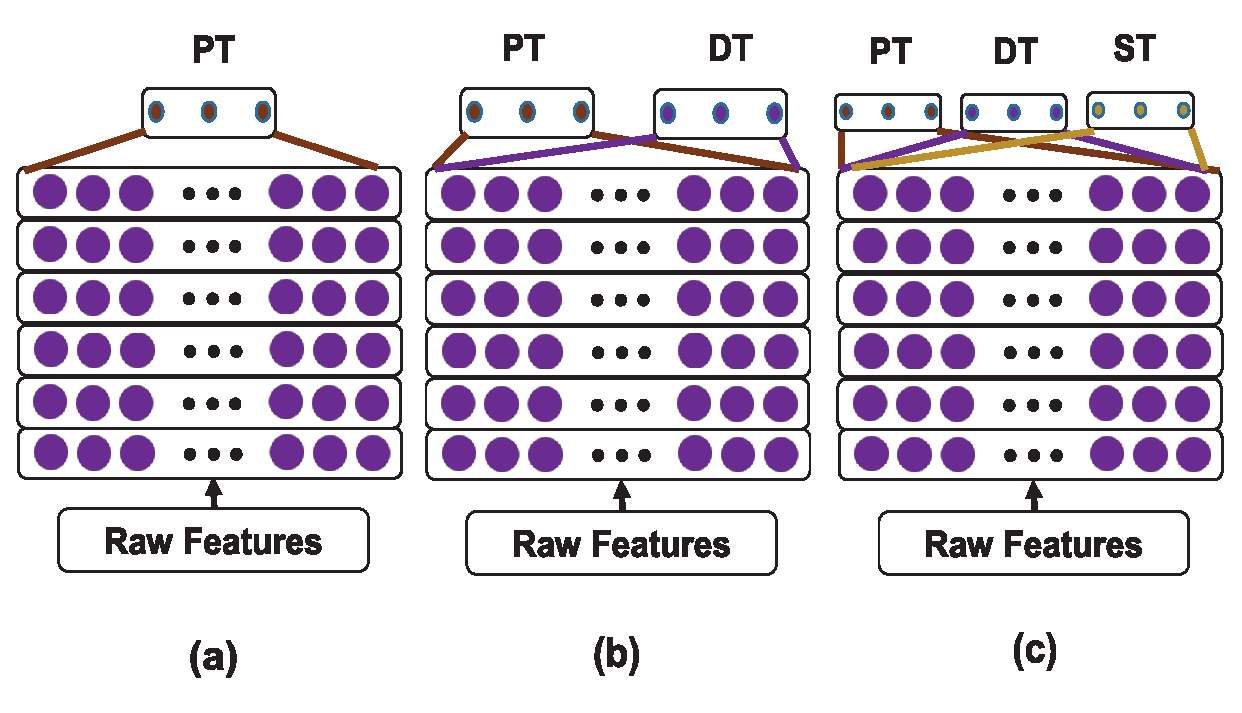
\includegraphics[width=\linewidth,height=5cm,keepaspectratio]{fig/DNN_multisoftmax.eps}
 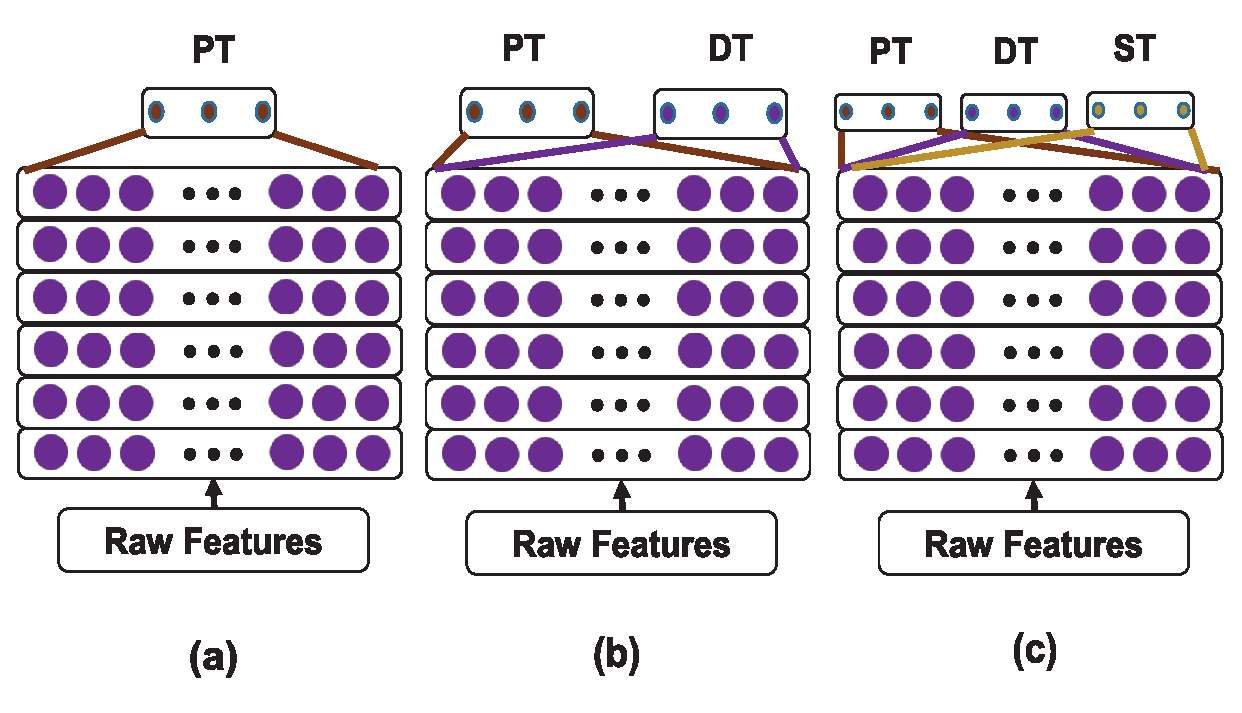
\includegraphics[width=\linewidth,height=5cm,keepaspectratio]{fig/DNN_multisoftmax.eps} 
 \caption{DNN adaptation to probabilistic transcripts (PT).}
 \myvspacefig
 \label{fig:DNN}
\end{figure}
%\end{wrapfigure}

\begin{comment}
\vspace{-4mm}
\begin{itemize}
\item Since the amount of multilingual training data is greater than the amount of monolingual data, the non-linear feature transformations learned by multilingual SHLs are better than those learned with monolingual data. \vspace{-4mm}
\item The SHLs of such a DNN are not biased to any particular language provided the amount of training data is uniform across all languages. Thus, the SHLs represent a ``global" view of the multilingual data. \vspace{-4mm}
\item Each softmax layer may be fine tuned to a specific language thus making it language dependent. Thus, the softmax layer represents a ``local view" of the multilingual data. \vspace{-4mm}
\item It obviates the need to explicitly map the phones to a common phone set. \vspace{-4mm}
\end{itemize}
\vspace{-4mm}
\end{comment}
\vspace{-2mm}
\section{Experiments and Results} \vspace{-1mm}
\label{sec:Experiments and Results}
In this section, we explore the effect of the three DNNs discussed in Section \ref{sec:DNN Training using Probabilistic Transcripts} in terms of PER. \vspace{-3mm}
\subsection{Data} \vspace{-2mm}
\label{sec:Data}
Multilingual audio files were obtained from the Special Broadcasting Service (SBS) network which publishes multilingual radio podcasts in Australia. These data include over 1000 hours of speech in 68 languages.
The following languages were used in our experiments - Swahili (swh), Hungarian (hun), Cantonese (yue), Mandarin (cmn), Arabic (arb), Urdu (urd). Out of these, the first three were used as target languages. %The podcasts were not entirely homogeneous in the target language and contain utterances interspersed with segments of music and English. An HMM-based language identification system was used to isolate regions that correspond mostly to the target language. These long segments were then split into smaller 5-second utterances. 
The utterances were short in length (5s) which makes it easy for crowd workers to annotate the utterances since they did not understand the utterance language. Each utterance was transcribed by 10 distinct Turkers and merged using \cite{Jyothi-MismatchedCrowdsourcingTrans} to create the PTs. More than 2500 Turkers participated in these tasks, with roughly 30\% of them claiming to know only English. The remaining Turkers claimed knowing other languages such as Spanish, French, German, Japanese, and Chinese.

Since English was the most common language among crowd workers, they were asked to annotate the sounds using English letters. The sequence of letters were not meant to be meaningful English words or sentences since this would be detrimental to the final performance. The important criterion was that the annotated letters represent sounds they heard from the utterances as if they were listening to non-sense syllables. The same set of utterances were labeled by native transcribers in the utterance language which constitute the DTs. This was required during ASR evaluations.

PTs and DTs, worth about 1 hour of audio, were collected from crowd workers and native transcribers respectively. The training set consists of a) about 40 minutes of PTs in the target language and, b) about 40 minutes of DTs in other source languages which exclude the target language. The development and test sets were worth 10 minutes each. As an example, if swh is the target language to be recognized, then the training set consists of 40 minutes of PTs in swh and 200 minutes of DTs in hun, yue, cmn, arb, and urd combined.

The orthographic transcriptions for the PTs and DTs were converted to IPA based phone transcriptions. The canonical pronunciation was derived from a lexicon. If a lexicon was not available, a language specific G2P model was used. To form a set of multilingual phone symbols, dipthongs/tripthongs were split into two/three indivudal phone symbols unless they were the same as English dipthongs. Diacritics such as tones and stress markers tend to make the phone symbols unique to a particular language.  Therefore, to enable phone merging across languages, such language specific diacritics were removed from the canonical phone transcriptions.

%This was followed by merging the phones to a reduced phone set. If an IPA phone symbol was unique in the sense that it appeared in the phone transcriptions of only one language, then that symbol was merged with another symbol which differs in only one distinctive feature. Repeating this process several times guarantees that each phone is represented in at least two languages. This enables sharing data across languages. The merged phone set is the multilingual or universal phone set. The total number of phones in the multilingual set (i.e., all languages from SW to UR) was 82 which excludes the silence phone.

Finally, phone based language models (LMs) were built from the text in the target language mined from Wikipedia. The corpus is summarized in Table \ref{Tab:Turkish and English Phoneme Set}. The test utterances were sufficiently shuffled so as to avoid biasing to a subset of speakers or to a specific gender.
\begin{table}
\begin{center}
\caption{SBS Multilingual Corpus.}
\label{Tab:Turkish and English Phoneme Set}
%\begin{tabular}{l|c c| c c| c}
%   \hline
%Language &  \multicolumn{2}{c|}{Utterances}  & \multicolumn{2}{c|}{Speakers} & Phones \\ 
%                 &  Train & Test  & Train & Test &  \\ \hline
%Swahili     & 463 & 123 & 14 & 4 & 53 \\ 
%Hungarian     & 459 & 117 & 52 & 14 & 70 \\ 
%Cantonese  & 544 & 148 & 34 & 19 &  37 \\ 
%Mandarin  & 467 & 113 & 25 & 6 &  57 \\ 
%Arabic  & 468 & 112 & 67 & 16 &  51 \\ 
%Urdu  & 385 & 94 & 20 & 5 &  45 \\ \hline
%Universal & - & - & - & - & 83 \\ \hline
%\end{tabular}
\vspace{-3mm}
\begin{tabular}{l|c c| c}
   \hline
Language &  \multicolumn{2}{c|}{Utterances}  & Phones \\ 
                 &  Train & Test &  \\ \hline
Swahili (swh)     & 463 & 123 & 53 \\ 
Hungarian (hun)    & 459 & 117 & 70 \\ 
Cantonese (yue)  & 544 & 148 &  37 \\ 
Mandarin (cmn) & 467 & 113 &  57 \\ 
Arabic (arb) & 468 & 112 &  51 \\ 
Urdu (urd) & 385 & 94 &  45 \\ \hline
All & - & - & 82 \\ \hline
\end{tabular}
\vspace{-5mm}
\end{center}
\end{table}
%  for L in SW HG AR UR MD CA; do  
%    wc -l data/$L/{train,eval}/wav.scp; 
%    wc -l data/$L/{train,eval}/spk2utt; 
%    wc -l data/$L/lang/phones.txt; 
%  done
\vspace{-0mm}
\begin{table}
\centering %\begin{center} does the same thing as \centering but inserts an extra line
\caption{PERs of monolingual HMM and DNN models. Dev set in parentheses.}
\vspace{-3mm}
\begin{tabular}{l|c c}
   \hline
Lang  & \multicolumn{2}{c}{PER (\%)} \\
          & HMM     & DNN   \\ \hline
swh        & 35.63 (47.00)   & 34.18 (39.49)   \\
hun        & 38.72 (40.33)   & 35.62 (37.32)   \\ 
%CA        & ???             & ???   \\ 
cmn        & 31.80 (26.14)   & 28.26 (25.16)   \\ \hline 
\end{tabular}
\vspace{-2mm}
\label{Tab:PER_Matched_Monolingual}
\end{table}
%for L in SW HG CA MD; do 
%  cat exp_$L/exp/monolingual/tri3b/$L/decode_*/scoring_kaldi/best_wer
%  cat exp_$L/exp/monolingual/dnn4_pretrain-dbn_dnn/$L/monosoftmax_dt/decode_*/scoring_kaldi/best_wer
%done

\begin{table}[t!]
\centering %\begin{center} does the same thing as \centering but inserts an extra line
\caption{PERs of multilingual HMM and DNN models. Dev set in parentheses.}
\vspace{-3mm}
\begin{tabular}{l|c c c}
   \hline
Lang  & \multicolumn{3}{c}{PER (\%)} \\
          &  HMM & DNN & \# Senones   \\ \hline
swh      &65.73 (67.58)   &61.17 (63.12) & 1003 \\
hun    &67.55 (68.50)   &63.25 (63.65) &  1012 \\ 
%CA    &69.64   &???   \\ 
cmn     &71.09 (69.10)   &64.68 (63.84) & 994  \\ \hline
\end{tabular}
\vspace{-2mm}
\label{Tab:PER_Mismatched_Multilingual}
\end{table}
% for L in SW HG CA MD; do
%  cat exp_$L/exp/tri3b/$L/decode_*_$L/scoring_kaldi/best_wer
%  cat exp_$L/exp/dnn4_pretrain-dbn_dnn/$L/monosoftmax_dt/decode_*_$L/scoring_kaldi/best_wer
% done

\begin{table}[t!]
\centering %\begin{center} does the same thing as \centering but inserts an extra line
\caption{PERs of self-trained DNN models trained using STs. Dev set in parentheses.}
\vspace{-3mm}
\begin{tabular}{l|c }
   \hline
Lang  & \multicolumn{1}{c}{PER \%} \\ \hline
swh   &  60.14 (62.07)  \\
hun   &  61.05 (62.26) \\
cmn   &  63.67 (61.94)  \\ \hline
\end{tabular}
\vspace{-6mm}
\label{Tab:PER_ASRPT_DNN_monosoftmax}
\end{table}
% for L in SW HG CA MD; 
%  do cat exp_$L/exp/dnn4_pretrain-dbn_dnn/$L/monosoftmax_asrpt_fw*/decode_*_text_G_$L/scoring_kaldi/best_wer; 
% done

\begin{table*}[t]
\centering %\begin{center} does the same thing as \centering but inserts an extra line
\caption{PERs of HMM, DNN-1, DNN-2, DNN-3 models trained using PTs. First element in parentheses is the PER of the dev set. Second element is the absolute improvement in PER of the test set over MAP HMM.}
\vspace{-3mm}
%\scalebox{1.0}{
\begin{tabular}{l|c c c c}
   \hline
Lang  & \multicolumn{4}{c}{PER (\%)} \\
        &MAP HMM       	   &DNN-1         		&DNN-2          &DNN-3                \\ \hline
swh      &44.77 (50.97,0.0) &45.14 (47.83,-0.37) &\bf{43.03 (45.87,1.74)}   &43.50 (45.95, 1.27)     \\
hun      &56.85 (57.69,0.0) &56.13 (57.21,0.72)  &\bf{55.53  (56.08,1.32)}  &55.69 (56.85, 1.16)     \\ 
cmn      &59.23 (58.05,0.0) &54.95 (54.35,4.28)  &53.70  (53.94,5.53)  &\bf{53.05 (53.59, 6.18)}     \\ \hline
%Avg.    &53.62 (         ) &52.07               &50.75                     &50.75 \\ \hline
\end{tabular}
%}
\vspace{-5mm}
\label{Tab:PER_PT}
\end{table*}
% MAP HMM
% for L in SW HG CA MD; do
%  cat exp_$L/exp/tri3c/$L/decode_*_$L/scoring_kaldi/best_wer
% done

% DNN-1 (1 softmax)
% for L in SW HG CA MD; do 
%  cat exp_$L/exp/dnn4_pretrain-dbn_dnn/$L/monosoftmax_pt/decode_*_text_G_$L/scoring_kaldi/best_wer
%  cat exp_$L/exp/dnn4_pretrain-dbn_dnn/$L/monosoftmax_pt_fw*/decode_*_text_G_$L/scoring_kaldi/best_wer
% done

% DNN-2 (2 softmax)
%  for L in SW HG CA MD; do
%   cat exp_$L/exp/dnn4_pretrain-dbn_dnn/$L/multisoftmax_pt_fw*_cop[0-4]/decode_block_1_*_text_G_$L/scoring_kaldi/best_wer
% done

% DNN-3 (3 softmax)
% for L in SW HG CA MD; do
%  cat exp_$L/exp/dnn4_pretrain-dbn_dnn/$L/multisoftmax_pt_fw*_cop*_unsup4000/decode_block_1_*_text_G_$L/scoring_kaldi/best_wer
% done






\vspace{-3mm}
\subsection{Monolingual HMM and DNN} \vspace{-2mm}
\label{sec:Monolingual HMM and DNN}
In the first baseline, monolingual HMM and DNN models were trained and tested using DTs in the target language. This is the oracle scenario if we assume DTs were to be available in the target language. Context-dependent GMM-HMM monolingual acoustic models were trained using 39-dimensional MFCC features which include the delta and acceleration coefficients. Temporal context was included by splicing 7 successive 13-dimensional MFCC vectors (current +/- 3 frames) into a high dimensional supervector and then projecting the supervector to 40 dimensions using linear discriminant analysis (LDA). Using these features, a maximum likelihood linear transform (MLLT) \cite{Gopinath-MLLT} was computed to transform the means of the existing model. The forced alignments obtained from the LDA+MLLT model were further used for speaker adaptive training (SAT) by computing feature-space maximum likelihood linear regression (fMLLR) transforms \cite{Gales-CMLLR}. The LDA+MLLT+SAT model is the final HMM model that will be simply referred to as HMM in all experiments. The forced aligned senones obtained from the HMM were treated as the ground truth labels for DNN training. 

For DNN training, we start with greedy layer-wise Restricted Boltzmann Machines (RBMs) unsupervised pre-training since this leads to better initialization \cite{Bengio-Pretraining}. Then the DNNs were fine-tuned using supervised cross-entropy training.  All experiments were conducted using the Kaldi toolkit \cite{Povey-Kaldi}. The monolingual PERs over a total of about 7K-8K phones  are given in Table \ref{Tab:PER_Matched_Monolingual}. This give us an estimate about the approximate lower bound PERs thereby indicating this is possibly the best we can achieve.
 \vspace{-3mm}
\subsection{Multilingual HMM and DNN} \vspace{-2mm}
\label{sec:Multilingual HMM and DNN}
Since the paper assumes zero DTs in the target language during training, in the second baseline, multilingual DTs were used to train HMMs and DNNs where the multilingual DTs \emph{exclude} the DTs in the target language.  The training procedure was the same as the one outlined in Section \ref{sec:Monolingual HMM and DNN}. The DNNs were trained using 6 hidden layers with 1024 nodes per layer. The total number of output nodes in the softmax layer representing multilingual senones was around 1000.  The PERs are given in Table \ref{Tab:PER_Mismatched_Multilingual}. Expectedly, due to lack of DTs in the target language, the PERs are much higher than the ideal case in Table \ref{Tab:PER_Matched_Monolingual}. Hence, the PERs in Table \ref{Tab:PER_Mismatched_Multilingual} establish the upper bound of PERs. In all subsequent experiments, we start from the upper bound of PERs in Table \ref{Tab:PER_Mismatched_Multilingual} and attempt to approach the lower bound PERs in Table \ref{Tab:PER_Matched_Monolingual}. 
\vspace{-3mm}


\subsection{Self-training DNN} \vspace{-2mm}
\label{sec:Self-training}
In this experiment, we explore a self-training algorithm \cite{Vesely-SemisupTrainingDNN} in which a multilingual ASR system decodes the audio in the target language and then uses the confidence selected decoded labels to retrain itself in the target language \cite{Knill-SelfTrainingAndUnsupAdapt}. The objective of this experiment is to evaluate the efficacy of the STs (self-training transcripts) vs PTs. Since we are interested in generating STs from an ASR, we ignore the PTs from crowd workers and decode the 40 minutes of audio in the training set using the multilingual DNN from Section \ref{sec:Multilingual HMM and DNN}. %Since the multilingual DNN is not trained in the target language DT, the decoded labels are very likely to be unreliable. Hence, we use only a subset of frames, selected by first evaluating the frame level confidences \cite{Vesely-SemisupTrainingDNN}. The confidences are simply the values of the posteriors of the best path in the decoding lattice. In the second step, an empirically determined threshold is chosen and compared with the frame confidences. Any frame whose confidence is above the threshold is selected for training. Otherwise, it is discarded. 
The results are given in Table \ref{Tab:PER_ASRPT_DNN_monosoftmax}. Compared to the multilingual DNN in Table \ref{Tab:PER_Mismatched_Multilingual}, the improvement due to self-training is in the range 1.01\%-2.20\%. We determined frame confidence thresholds as 0.5 or 0.6 from the development set. 
\vspace{-3mm}
% Tell about estimation of priors using feed forward if you have space

\subsection{Training one softmax DNNs using PT: DNN-1} \vspace{-2mm}
\label{sec:Effect of training single softmax DNNs using crowdsource PT data}
In this experiment, we use PT labels from crowd workers to train the DNN-1 system in Fig.~\ref{fig:DNN}(a). In the first step, the multilingual HMM models in Section \ref{sec:Multilingual HMM and DNN} are adapted to the PTs using MAP adaptation. Details of this step are given in \cite{Liu-PTAdaptedGMM}. The PER results for the MAP adapted HMM are given in the first column of Table \ref{Tab:PER_PT}. The absolute improvement in PER over multilingual DNN models in Table \ref{Tab:PER_Mismatched_Multilingual} is significantly higher than self-training, in the range 5.45\%-16.4\%. The conventional way to adapt a DNN using DTs is to retain the SHLs of the multilingual DNN, replace the existing softmax layer with a single randomly initialized layer and fine tune this new layer using 1-hot senone alignments from an HMM \cite{Ghoshal-MultilingualPretraining}. Here, for the case of PTs, the MAP adapted HMM generates soft alignments of the PTs which are used for fine tuning the new softmax layer. The results for DNN-1 are given in the second column of Table \ref{Tab:PER_PT}. Since the DNNs are now tuned to the target language PTs, we compare their performance with MAP adapted HMMs. The absolute improvement is in the range -0.37-4.28. Clearly, DNN-1 performed worse than MAP HMM for Swahili and the improvement is marginal for Hungarian. Thus, DNN-1 exhibits chance performance. Hence, this approach does not work very well for PTs largely due to the presence of incorrect labels in PTs.
\vspace{-3mm}
\subsection{Training two softmax DNNs using PT and DT: DNN-2}  \vspace{-2mm}
\label{sec:Effect of training two softmax DNNs using crowdsource PT and multilingual DT data}
In this experiment, instead of using a single softmax layer, we use two separate softmax layers illustrated as the DNN-2 system in Fig.~\ref{fig:DNN}(b). The first softmax layer is trained with target language PTs only whereas the second softmax layer is trained with multilingual DTs. While training DNN-2, we find introducing an additional copy of the multilingual DTs may sometimes lead to better PERs. This was observed in the case of Hungarian. For the other two languages (Swahili and Mandarin), additional copies were not required. We determined the number of copies from the development set. The results are given in the third column of Table \ref{Tab:PER_PT}. This time the improvement in PERs over MAP HMM is consistent and significantly higher (1.32\%-5.53\%) than the improvement in DNN-1.
\vspace{-3mm}
\subsection{Training three softmax DNNs using PT, DT, and ST: DNN-3} \vspace{-2mm}
\label{sec:Effect of training three softmax DNNs using crowdsourced PT, multilingual DT, and unsupervised data}
In this experiment, we introduce a third softmax layer (see Fig.~\ref{fig:DNN}(c)) for ST labels generated from decoding additional unsupervised data in the target language (4000 utterances $\sim$ 5.5 hours) using the DNN-2 system. We use the DNN-2 to decode unsupervised data instead of the multilingual DNN since the former is better adapted to recognize the target language. Hence, the languages of PTs and STs are matched. Frames which had confidences below a threshold of 0.9 were discarded since frames above this threshold are expected to have reliable labels. To balance the effect of disproportionate amounts of data between the DTs and STs, we created multiple (2-4) copies of the frames labeled with DTs where the number of copies were determined from the development set. The PER results are presented in Table \ref{Tab:PER_PT}. The results are similar to DNN-2 with improvements in the range 1.16\%-6.18\% . It appears that DNN-3 is not significantly better than DNN-2 but still outperforms DNN-1. Perhaps decoding more unsupervised audio to generate more STs or adding the STs to the PTs and then retraining using the DNN-2 architecture might be useful. This is currently under investigation.


Finally, comparing the PERs in Table \ref{Tab:PER_ASRPT_DNN_monosoftmax} (self-train), Table \ref{Tab:PER_PT} (DNN adapted) with the lower and upper bound PERs listed in Table \ref{Tab:PER_Matched_Monolingual} (monlingual) and Table \ref{Tab:PER_Mismatched_Multilingual} (multilingual) respectively, three findings are evident. %First, PTs are not as useful as DTs: the gap between Table \ref{Tab:PER_Matched_Monolingual} and Table \ref{Tab:PER_PT} is still large. 
First, from Table \ref{Tab:PER_PT}, DNN-2 or DNN-3 outperform DNN-1 and MAP-HMM systems. Thus, for PTs, we recommend DNN-2/DNN-3 as reliable baselines for adapting DNN to PTs instead of the conventional adaptation in DNN-1. Second, DNN-2/DNN-3 are able to close between 28\% and 67\% (relative) of the gap between Table \ref{Tab:PER_Mismatched_Multilingual} and Table \ref{Tab:PER_Matched_Monolingual}. Thus, we can say that PTs are between one and two thirds as useful as DTs. Third, PTs from crowd workers are more useful than STs generated from an ASR system (Table \ref{Tab:PER_PT} vs Table \ref{Tab:PER_ASRPT_DNN_monosoftmax}).
%SW: 100*(61.17-43.03)/(61.17-34.18) = 67.21 %   (2 softmax)
%HG: 100*(63.25-55.53)/(63.25-35.62) = 27.94 %   (2 softmax)
%MD: 100*(64.68-53.05)/(64.68-28.26) = 31.93 %   (3 softmax)

%\vspace{-0mm}
\section{Conclusions} \vspace{-1mm}
We investigated multiple DNN training strategies to adapt DNNs to probabilistic transcripts collected from crowd workers not familiar with the target language. We demonstrated that adaptation to probabilistic transcripts using the conventional DNN-1 system is not reliable. As a result, we proposed adaptation using DNN-2 or DNN-3 systems which consistently outperform DNN-1 and HMM systems. The absolute PER improvement for 3 languages were in the range 1.3\%-6.2\%.

%\vspace{-0mm}
\section{Acknowledgements}  \vspace{-1mm}
The work reported here was started at the JSALT 2015 workshop in the University of Washington, Seattle and was partly supported by the Johns Hopkins University via grants from Google, Microsoft, Amazon, Mitsubishi Electric, and MERL. The authors thank Paul Hager, Massachusetts Institute of Technology and Karel Vesel\'y, Brno University of Technology for discussions.

% To start a new column (but not a new page) and help balance the last-page
% column length use \vfill\pagebreak.
% -------------------------------------------------------------------------
%\vfill
%\pagebreak

\clearpage
\newpage
\eightpt
\bibliographystyle{IEEEtran}
\bibliography{IEEEabrv,IEEEexample}

%  \begin{thebibliography}{9}
%    \bibitem[1]{Davis80-COP}
%      S.\ B.\ Davis and P.\ Mermelstein,
%      ``Comparison of parametric representation for monosyllabic word recognition in continuously spoken sentences,''
%      \textit{IEEE Transactions on Acoustics, Speech and Signal Processing}, vol.~28, no.~4, pp.~357--366, 1980.
%    \bibitem[2]{Rabiner89-ATO}
%      L.\ R.\ Rabiner,
%      ``A tutorial on hidden Markov models and selected applications in speech recognition,''
%      \textit{Proceedings of the IEEE}, vol.~77, no.~2, pp.~257-286, 1989.
%    \bibitem[3]{Hastie09-TEO}
%      T.\ Hastie, R.\ Tibshirani, and J.\ Friedman,
%      \textit{The Elements of Statistical Learning -- Data Mining, Inference, and Prediction}.
%      New York: Springer, 2009.
%    \bibitem[4]{YourName16-XXX}
%      F.\ Lastname1, F.\ Lastname2, and F.\ Lastname3,
%      ``Title of your INTERSPEECH 2016 publication,''
%      in \textit{Interspeech 2016 -- 16\textsuperscript{th} Annual Conference of the International Speech Communication Association, September 8–12, San Francisco, California, USA, Proceedings, Proceedings}, 2016, pp.~100--104.
%  \end{thebibliography}

\end{document}
